\section{Compiler structure \rr}
The \lan compiler is structured into different modules that can be seen in figure
\ref{fig:compiler-overview}. First the \lan source code is handed as input to the frontend,
which creates an abstract syntax tree (AST), that is then type checked and annotated with
context sensitive information. This annotated AST is then reversed, giving us a reversed AST
$R(AST)$ and the regular. These two trees are then run through the optimizer, that outputs
two optimized trees, that is then translated into \texttt{C++} output via standard out.

\begin{figure}[h!]
    \centering
    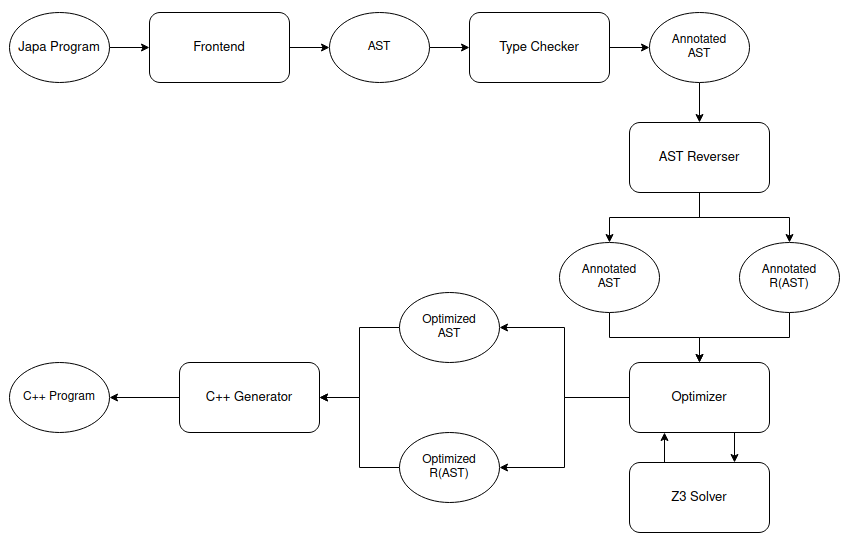
\includegraphics[scale=0.6]{imgs/compiler-overview.png}
    \caption{Compiler structure overview.}
    \label{fig:compiler-overview}
\end{figure}

\subsection{Frontend \rr}
% Theory and information behind lexing and parsing
The frontend consists of a lexical analysis and a syntax analysis. Both are implemented using a
parser combinator in \texttt{Haskell}, namely Parsec. A parser combinator is a higher-order
function taking in a parser as input, and outputting another parser. This way small simple parsers
can be combined into more complex structures, thereby helping quick prototyping. This strong
functionality does however come with a significant overhead, especially considering the simplicity
of \lan \cite{parser}.

The strong flexibility of parser combinators, and their strong resemblance of the underlying
grammar does however outweigh the negativity of the performance, especially considering this is
not the primary focus of this bachelor thesis.
\\
\\
Because the language is not in LL(1) the performance of the parser is also worsen, as lookahead
cannot be avoided e.g. in the distinction between simple variables and arrays, and the two
kinds of for-loops. The process presented in \cite{torben} can be used to transform it into
LL(1), but due to time constraints, this has been postponed to future works.
\\
\\
The parser combinator works on a string input on which it performs intertwined lexical analysis
and syntax analysis. The two analysis' are intertwined simply because that is how the Parsec
library functions. This does not pose any apparent problems, as the language being analyzed has
a fairly simple syntax. Parsec does however still keep a sense of modularity.

\subsection{Type checker \rr}
% Theory and information behind type checking
\lan is a statically typed language, as the type check is performed before execution of the program.
Furthermore, it is a strongly typed language, as operations are ensured to be performed on
types that are supported. The reason to make \lan a strongly typed language, as opposed to
the more weakly typed \texttt{C++}, which it is translated into, is that a strongly typed
language gives run-time guarantees that helps avoid certain type of program errors, that can be
hard to pinpoint during debugging, and even worse, might not even show up.
\\
\\
While type checking the AST two mappings are used to carry the type information synthesized by the
recursive calls onwards, so that the information can be inherited in other part of the AST; this
is a mapping from variable names to types, and from variable names to size. The latter is used
to annotate the AST with array sizes, that is needed during the subsequent optimizer phase.
No guessing of types are done during the analysis, meaning when an error is met it is reported
and the analysis stops.

\subsubsection{Type checking expressions}
When type checking expressions the symbol tables for variables and array size are inherited
attributes, and the type of expression, together with a annotated expression,
is the synthesized attributes. The rules for type checking
can be summarized as:

\begin{itemize}
    \item A number is simply an integer.

    \item A boolean value is a bool.

    \item The type of a variable is found by a lookup in the inherited variable table.
          If the lookup is successful the type is returned back, and if it fails a error
          is reported.

    \item The type of a lookup in an array is also determined by a lookup in the variable table.
          However, for array lookup the size needs to be annotated onto the expression, meaning
          a lookup into the array table is performed. If both are successful it is checked
          whether the array indexing is integers. If so the annotated
          expression is returned together with the type. Else an error is reported.

    \item For binary operations the type of the two expressions must match. As all types
          are defined for all operators, if the two types match the operator is checked in order
          to know what type it returns. If it is a boolean operator, the possibly annotated
          expression is returned together with the boolean type. Else the type of the expression
          is returned together with its annotated self. The choice that plus and multiply
          functions also for booleans is simply because \texttt{C++} does so.
        
    \item The type of the \lsin{not} expression is always boolean. Meaning the expression
          being inverted is simply checked, and then the possibly annotated expression is
          returned with the boolean type.

    \item The \lsin{size} expression always returns an integer, so the expression is simply
          returned with the integer type.
\end{itemize}

\subsubsection{Type checking statements}
Type checking statements involve the same inherited attributes, but here the synthesized are
the type/size annotated statement, and the updated tables.
The rules for type checking statements can be described as:

\begin{itemize}
    \item Variable definition and deallocation explicitly declare which type they are. Hence
          the check merely involves type checking the assigned expression, and see if it matches
          the declared type. If not an error is reported. Else the updated tables are returned
          together with annotated statement.

    \item For both simple types and arrays, the modification expression is checked if it matches
          the moderated variable. Array types the indexing expressions are also checked
          to be integers. If all is true, the updated tables are returned together with
          the now annotated statement. Else an error is reported.      

    \item A switch statement need to switch between two equal variables; so the types must match
          and if it is between arrays, the size of the arrays must also match. If these are not
          true, an error is reported, else the annotated statement together with the updated
          tables are returned.

    \item In conditional branching (if-then-else) both the if conditional, and the fi conditional
          must be a boolean type. Because these are statements and not expressions, the two
          branches do not have any "return" type, meaning the conditional rules are the only.
          So if they are true, the branch bodies are type checked, and the annotated statement
          is returned together with the inherited tables. Else an error is reported.

    \item In for loops the declaration, moderation, and deallocation needs to be type checked
          as explained above. Furthermore, the possible invariant needs to be a boolean type.
          If all that is true, the body is type checked, and an annotated statement is returned
          together with the inherited tables.

    \item Assertions simply needs to be a boolean type. If true the annotated statement is returned
          together with the inherited tables.
\end{itemize}


\subsubsection{Type checking procedure definitions}
Each procedure inherits the global store attributes, and uses this to type check its arguments,
and procedure body. Because there are no return types of procedures, it is only the arguments and
body, that needs type checking.

When all procedures have been type checked, the annotated AST is returned and used in the
subsequent phases of the compiler.

\subsection{AST reversing \rr}
The reverser simply follows the rules outlined under \nameref{sec:language-def}. The AST is
reversed at this point in the compiler, as the optimization checks needs to be performed for both
direction as explained in \ref{translation-to-z3}.

After the reversal each procedure should occur in the same order in the AST, but each
procedure body should be reversed. To achieve this the right associative \lsin{foldr} is used to
go through each procedure, and the left associative \lsin{foldl} is used within each procedure.
This can be seen in listing \ref{lst:reverser}. Notice that the first procedure in the AST is
skipped. This works under the contract, that the first procedure is always the \lsin{main}
procedure. The \lsin{main} procedure is not reversed because, it is used to define the start state
of the program. Hence it contains the global variables, which can only we 'reversed' if one were
to know the end state of the program, which would defeat some of the purpose of actually writing
the program in the first place.

\begin{lstlisting}[language=Haskell, label={lst:reverser}, caption={Reversing AST.}]
reverseProcedure (ProcDecl name args body pos) acc =
      let body' = foldl reverseStatement [] body in
            ProcDecl name args body' pos : acc

reverseProgram (Program ps) =
      let m = head ps in
            let rest = foldr reverseProcedure [] (tail ps) in
                  Program $ m:rest
\end{lstlisting}
\noindent
The methods for reversing statements are implemented as outlined in \nameref{sec:language-def},
but the implementeation for if-statements and for-loops will be descriped further here. These
can be seen in listing \ref{lst:stmt-reverser}. If-statements have their two conditionals switched,
such that the entrance conditional becomes the exit condition (from if path) and vice verser.
Then both paths are reversed recursively. With for-loops the expression of the loop variable at
entrance, is exchanged with the expression for the exit condition. Then the body is recursively
reversed.

Exchaning entrance and exit conditionals for the two constructs, guarantees that the reversed
statements bodies, will only be executed, if they were executed during the forward run. This
is illustrated in figure \ref{fig:rev-flow-constructs}; where reversal of the graph is done
by converting Diamonds to circles. circles to diamonds, squares to reversed squares, and at
last changing the arrows direction. Note that the reversible loop construct requires, that
the entrance condiotional be true, whenever the statement is executed. This is guaranteed in
\lan by using the for-loop construct instead of the from-loop, thereby making it possible to
exclude that runtime check.

\begin{lstlisting}[language=Haskell, label={lst:stmt-reverser}, caption={Reversing for-loops and if-statements.}]
reverseStatement acc = \case
      ...
      Ite condif bodyif condfi bodyelse pos ->
            Ite condfi
            (foldl reverseStatement [] bodyif)
            condif
            (foldl reverseStatement [] bodyelse)
            pos
            : acc

      For1 inv (Var t n (Just e) p) body mod cond b pos ->
            For2 inv (Var t n (Just cond) p) (reverseMod mod)
            (foldl reverseStatement [] body)
            e b pos
            : access
      For2 inv (Var t n (Just e) p) mod body cond b pos ->
            For1 inv (Var t n (Just cond) p)
            (foldl reverseStatement [] body)
            (reverseMod mod) e b pos
            : acc
      ...
\end{lstlisting}

\begin{figure}[H]
      \centering
      \begin{subfigure}[b]{0.4\textwidth}
            \centering
            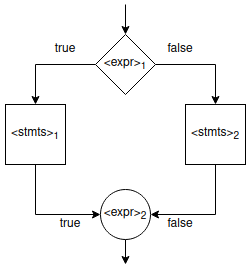
\includegraphics[scale=0.5]{imgs/reversible-conditional.png}
            \caption{Conditional.}
      \end{subfigure}
      \hfill
      \begin{subfigure}[b]{0.4\textwidth}
            \centering
            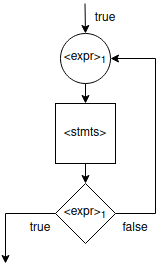
\includegraphics[scale=0.5]{imgs/reversible-loop.png}
            \caption{Loop.}
      \end{subfigure}
      \caption{Reversing conditionals and loop constructs.}
      \label{fig:rev-flow-constructs}
\end{figure}

\subsection{Optimization \rr}
% Strategy for optimization
% Integration with theorem prover
Because the compiler translates directly from the source language into an abstract syntax tree,
and then into \texttt{C++}, the optimization must be done on the abstract syntax tree, as it is
the easiest data structure to work on of the three. Doing the optimization directly on the source
language itself, saves the computation of translating to some intermediate language, but does
make this optimizer local to the source language.
\\
\\
This optimization involves four steps:
\begin{enumerate}
    \item Discovering language constructs, that require run-time assertions.
    \item Locating and gathering information for the prover.
    \item Translation of abstract syntax tree into \texttt{z3}.
    \item Deciding on whether to optimize the assertion or not, based on the answer
          from \texttt{z3}.
\end{enumerate}

\subsubsection{Language constructs requirering runtime assertions \rr}
The first point can be discovered by consulting the language specification introduced
in section \ref{sec:language-def}. Here it is imminent, that the following construct introduce
assertions for the translated code:
\begin{itemize} % TODO: Give example showing where assertions are created
    \item Deallocation of local variables.
    \item If statement as the program needs to know whether the if-path was chosen or not when
          reversing computations.

    \item For statement as the initial loop state must only be true at the initialization of the
          loop and never hereafter. This is the case, as it will function as the loop end
          condition, when reversing the statement.

    \item Assertions as it is in their nature.
\end{itemize}
\noindent
Which means that when running through the abstract syntax tree, the optimizer must stop and validate
when the above constructs are met, and then decide on whether to optimize based on the answer from
\texttt{z3}.

\subsubsection{Gathering information for \texttt{z3} \rr}
% Write more inticate details on loops e.g. how isdescending works, and how unroll works by using satisfy instead of validate
Point two has two main obstacles: 1) to know how much information \texttt{z3} needs for the proof,
and 2) granting the optimizer access to this appropriate subtree.

For 1) a simply approach could be to give the tree representing the current procedure to the
optimizer. This could give too much information in the sense that only part of this subtree is
actually needed to perform the validation check. e.g. in the small program, in listing
\ref{listing:z3-info-gather-ex}, the only thing
needed for the validation is the two last lines. However, this would require backtracking the
tree while keeping a list of "unassigned" variables, until this list is empty, so the first
method is used in this optimizer. For future work, it would be a good idea to check whether the
other approach would be faster. The below piece of code also reveal two other problem in regards
to information: Global variables and procedure calls.

To address this problem, the global store is processed before any optimization is performed.
In this way all procedures have access to this global store. \lan is statically scoped meaning
only the global store is available across procedures; this is the case as all procedures are
defined as the first thing in the program.
\\
\\
The information gathering is simply done locally for each procedure. Meaning when optimizing
a procedure \lsin{foo}, the only prior information is the global store. Then when a procedure
call for \lsin{bar} is met, \lsin{bar} is processed, so its information is carried out into
the analysis of \lsin{foo}. While doing this processing of \lsin{bar}, no optimization is done,
as that would use information from the call site, which could lead to spurious optimizations.
Because procedures are non-recursive this "inlining" can be done trivially without further
analysis.

\begin{lstlisting}[language=C++, label=listing:z3-info-gather-ex,
    caption=Example on gathering information for \texttt{z3} where only last two lines are needed.]
    int c

    procedure g()
    {
        c += 5
    }

    procedure f(int a)
    {
        call g()
        a += c
        local b = 1
        delocal b == 1
    }
\end{lstlisting}

\subsubsection{Handling if-then-else and for loop optimization \rr}
Conditional control-flow statements are the most complex to do a optimization run on, so they
will be explained further in the next two subsections.
\\
\\
\textbf{If-then-else}: As explained and outlined in section \ref{translation-to-z3}, the optimizer
cannot know statically which branch is going to be taken at run-time (at least for other than
trivial programs). Hence the translation must happen through the \texttt{z3} function
\lsin{mkIte}.

This function works by modelling each branch flow, and then "hiding" them both behind the
conditional decider. The code for this can bee seen in listing \ref{listing:ite}. What it does
is, that for each variable in the scope coming into the if-then-else, the variable is checked
in the two branches scope (the modeling of these scopes are processes prior to this) of whether
they have been "invalidated" by being removed (invalidation will be covered under loops below).
Then \lsin{mkIte} is used to base the decision on the variables value in the scope on the
if-conditional.

\begin{lstlisting}[language=Haskell, label=listing:ite, caption=Using \lsin{mkIte}.]
createITE :: AST -> Vars -> Vars -> Vars -> Z3 Vars
createITE cond orig scope1 scope2 = foldM f orig $ Map.keys orig
    where f scope name = do
            let var1 = tryGetVar name scope1
            let var2 = tryGetVar name scope2

            case (var1, var2) of
            (Just (var1z3, var), Just (var2z3, _)) -> do
                newVar <- makeVar (fromJust (getVarType var)) name
                ite    <- Z3.mkIte cond var1z3 var2z3
                Z3.assert =<< Z3.mkEq newVar ite
                return $ Map.insert name (newVar, var) scope

            -- else variable invalidated in some scope
            _ -> return $ Map.delete name scope
\end{lstlisting}
\noindent
\textbf{Loops}: \texttt{Z3} does not have a theory for handling loops. A loop must therefore be
reformulated for \texttt{z3}, as mentioned in section \ref{translation-to-z3}. The optimizer
has three different cases in which some information can be transferred to \texttt{z3}: 1)
Loop has invariant attached and can be unrolled, 2) loop cannot be unrolled but has invariant,
and 3) loop does not have an invariant attached but can be unrolled. For all other combinations
it is, to the best of my knowledge, not safe to carry information to \texttt{z3}, as we cannot
paint the whole picture. An example for this is, if it is conveyed that $x = c_1$ to \texttt{z3}
prior to the loop, and the loop would ensure $x=c_2$, but we have no way of statically getting this.
If the information of $x=c_1$ was then carried on past the loop, it could result in faulty
optimizations. Invalidating $x$ is done by replacing the \texttt{z3} var representing the value
of $x$, by a new \texttt{z3} variable, of which we know no more than it's existence; this way
no prior information, which now may be invalid, is carried onwards in the analysis.

Determining whether loops are unrollable is done with the simple method, of 
\begin{enumerate}
    \item Checking that the initial value, the loop modifier, and the deallocation are based on
          simple constants.

    \item No modification of the loop variable should be performed during the loop body execution.

    \item The loop should not be based on integer overflow/underflow.

    \item The loop unroll number does not exceed an arbitrary given bound (simply to not let
          the recursively loop "forever").
\end{enumerate}
\noindent
If all above criterions are met, the loop is deemed unrollable, and the loop will be unrolled.
Otherwise all modified variables within the loop are invalidated, except for those in
the loop invariant.

In order for an invariant to help carry information past a loop that cannot be unrolled, it needs
to be true at initialization of the loop, during maintenance, and the loop should terminate.
The three criterions are validated by:
\begin{itemize}
    \item \emph{Initialization} is simply proved by validating the invariant before the loop starts.

    \item \emph{Maintenance} is proved by processing a run of the body and modification, on a
          generalized scope, and then validating the invariant. If the invariant is true for this
          general case, it will be true for all iterations. The generalization of the scope is
          done by "invalidating" the entire scope.

    \item \emph{Termination} is proved by validating that after a general run of the loop,
          the loop variable will be either strictly larger or smaller than before, depending
          on the loop modifier.
\end{itemize}
\noindent
Loop unrolling is only done to enable exact information for the \texttt{z3} solver. It has nothing
per se to do we the speed of the resulting code (ignoring the fact that missing information
might lead to assertions not being removed). Therefore, if the optimizer is given a nested loop,
if the inner loop cannot be unrolled, there is no use in unrolling the outer loop. Information will
be invalidated no matter what. Furthermore, as a matter of running time for the optimizer, there
is an arbitrary bound of the amount of unrolling done. Meaning if a loop requires 31 unrolls, but
the max is 30, the loop is not unrolled. Hence the inner loop is unrolled first, and then the outer
loop. If the inner loop requires 10 unroll, and the outer can be unrolled 5 times, the total
required unrolling of the outer is $10*5$. To further lessen the burden on the \texttt{z3}
solver, the function \lsin{satisfiable} is used instead of \lsin{validate} for the loop
variable assertions. This is the case, as the semantics of \lan forces this generated assertion
to be non bogus, meaning it is not needed to do the additional check of whether the expression
is bogus.
\\
\\
If a loop is deemed to not be unrollable, a generalized analysis of the loop will be performed.
This means the loop optimizer will be run on a generalized scope. The code snippet
\ref{require-generalize} shows an example, where this generalization is necessary to get the
correct result. If it was run once in the normal scope, the if path would not be considered,
meaning the for-loop would be optimized. But if \lsin{tmp} and \lsin{i} is generalized, the
optimizer will correctly state, that the loop is not optimize-able.
Generalizing the scope is done for all variables, that are modified within the loop body;
this also includes the loop variable.

\begin{lstlisting}[language=C++, label=require-generalize, caption=Loop requirering generalization]
int tmp = 0
for local int i = 0 {
      if (i == 3 && tmp == 0) {
            i -= 3
            tmp += 1
      } fi (i == 0 && tmp == 1)
} i += 1, until (dealloc int i = 4)
\end{lstlisting}
\noindent
This loop optimization based on a generalized scope can be seen in listing
\ref{lst:generalizeLoopOpt}.
First every variable that will be modified within the loop body is generalized, for the
reasons explained above. Then the compiler tries to validate whether the loop variable is
increasing or decreasing. This is used in order to put in more information about to loop
variable for the generalized run. If this step was omitted, many optimization could not be
done, as the generalized loop cannot guarantee that the loop variable does not overflow/underflow.
Hence guaranteeing that the loop variable will never reach the initial value again at the end
of an iteration becomes almost impossible; without the information from the
\lsin{loopDescending} call.
Then the statement body is optimized (if we are running optimization round), 
by calling \lsin{unroll} with \lsin{doOpt}. This then reveals whether the assertion
created by the loop variable, can be optimized away in a generalized environment.

\begin{lstlisting}[language=Haskell, label={lst:generalizeLoopOpt},
      caption={Optimizing the loop based on generalized information.}]
generalizedAnalysis scope body z3expr m state warnings = do
      -- Generalize all variables in scope, and check for validity
      tmpScope <- invalidateVars scope $ modifiedVars ast body

      -- Trying to get more information about the loop variable
      let loopVar = fst $ fromJust $ tryGetVar name tmpScope
      loopDirection <-
            loopDescending scope forward var m body state bound warnings
      (case loopDirection of
            Ascending  -> Z3.assert =<< Z3.mkBvuge loopVar z3expr
            Descending -> Z3.assert =<< Z3.mkBvule loopVar z3expr
            Unknown    -> return ())

      (body', _, validated, warnings') <-
            unroll 1 doOpt forward body pos var z3expr m tmpScope state warnings
      return (tmpScope, body', validated, warnings')
\end{lstlisting}

\subsection{Translation to \texttt{C++} \rr}
The \lan compiler presented in this report does a simple translation to \texttt{C++}.
As the focus lie on assertion removal, no work has been put into compiling effective
\texttt{C++} code. The main function of the code generator can be seen in listing
\ref{lst:formatMain}. It works by receiving two AST's: One forward direction and one reversed.
It starts by inserting includes possibly required by the translated code. This includes

\begin{itemize}
      \item \lsin{assert.h} to enable use of asserts in the \texttt{C++} code.

      \item \lsin{cstring} to get access to \lsin{memcmp} functionality, which is used
            when deallocating array variables.
\end{itemize}
\noindent
Then it formats the starting global store of the \lan program. This is put into the global
scope, so that they can be accessed freely from all functions. Because the main procedure of
the \lan program, is not reversed, it simply takes the one obtained from the forward AST
(here the first parameter).

Then function definition is created for all procedures of the program. This is done as
functions in \texttt{C++} can only be called after their declaration, whereas in \lan
they can be called, as long as they are in the global scope.
After this all procedures are formatted into \texttt{C++}.

\begin{lstlisting}[language=Haskell, label={lst:formatMain}, caption={Formatting AST into \texttt{C++}}]
formatProgram :: Program -> Program -> Doc
formatProgram (Program ps) (Program psR) =
      case zip ps psR of
      (main:tl) ->
      formatIncludes
      $+$ space $+$
      formatGlobalVars (getProcDeclBody (fst main))
      $+$ space $+$
      foldr formatProcedureDefinition empty tl
      $+$ space $+$
      foldr formatProcedure' empty tl
      $+$
      formatProcedure (fst main)
      [] -> empty
\end{lstlisting}
\noindent
Formatting procedure declarations are straight forward, as every procedure must return void.
The only thing is, that parameters are all passed by reference instead of values; for
normal variables this allows to alter the value within it; for arrays is avoids decaying the
variable to a pointer to first element. Decaying to a pointer is avoided, so the function
\lsin{sizeof} can still be used, even on array parameters. If the array was passed as value,
it would be decayed to \lsin{int*} meaning \lsin{sizeof} would return $8$ (depending on the
architecture).
\\
\\
When transforming the different statement constructs into \texttt{C++}, the following rules
are implemented:
\\
\\
\textbf{Local variables declaration, modification, and deallocation:}
Local variable declaration and modification are simply translated into regular variables and
assignment modifications in \texttt{C++}, as they behave
similarly. The only difference is, that \lan local variables needs to be deallocated at some
point. This deallocation is translated into \texttt{C++} assertions, as they behave as a
program runtime check.

deallocation of arrays are somewhat more complicated, as arrays in \texttt{C++} cannot be
declared inline in an assert. Hence a temporary array $_tmp_arr$ is created, with the values
stated in the deallocation statement, and is compared to the values of $arr$, by using
\lsin{memcmp}; as \lsin{memcmp} has no check for array length, this is checked before the
call, using the short-circuiting operator $\&\&$.
\\
\\
\textbf{Switch:}
At the moment switch statements are translated into a series of exclusive-or bitwise operations.
This is faster than creating a temporary variable to hold, the value of one of the variables, 
while during the switch. However, it does alter the behavior if the two variables being
switched aliases each other. Here the exclusive-or operations will simply zero-initialize
the two variables, instead of switching the values. This should be altered in the future,
unless guarantees can be made that the variables are non-aliasing.
\\
\\
\textbf{If-then-else:}
The only semantic difference between \lan conditional statements and \texttt{C++} ones,
is the runtime assertion from the \lsin{fi}, that should be true whenever the \lsin{if}
branch has been run. Hence the translation simply involves, transforming to a simple
\texttt{C++} if statement, with accompanying assertion of the \lsin{fi} expression, in the
if-branch.
\\
\\
\textbf{For loops:}
\lan for-loops are transformed into a while-loop. While-loops are chosen instead of for-loops
as \lan for-loops can alter whether the loop variable should be modified at the start of an
iteration or at the end. During the translation assertions can occur at the following
destinations:
\begin{enumerate}
      \item \label{en:init} After loop variable initialization, if there is an invariant and it isn't proven.
      \item \label{en:main} At the start loop body, if an invariant is given and not proven.
      \item \label{en:body} At the end of the loop body if loop could not be proven
      \item \label{en:term} After the loop construct, if invariant is present and not proven.
\end{enumerate}
\noindent
In order to keep track of which assertions should be formatted, and which have been proven
away, the data construct \lsin{data LoopInfo = LoopInfo Bool Int}. The bool indicates whether
assertion \ref{en:body} above should be present or not. All invariant based assertions are
tracked via the \lsin{LoopInfo} integer; the least significant bit indicated whether
assertion \ref{en:init} should be formatted; the next whether assert \ref{en:main} should
be formatted; the next whether assertion \ref{en:term} should be present. If the bit is
$1$ the invariant assertion should be formatted, else it has been proven always valid.